%! TeX program = lualatex
\documentclass[../main.tex]{subfiles}
\begin{document}
\begin{lesson}{Applied optimization problems}
  To optimize is to find the absolute maximum or absolute minimum of some function. The mathematical idea of modern machine learning (or AI) is to find a function (given some known data set) that \emph{minimizes} certain type of error measurement. The resulting function is used to \emph{predict} the future.

  Optimization problems are good opportunities to work on our problem-solving skills. A combination of geometry, algebra skills and differential calculus usually go into solving an optimization problem.

  \bigskip
  Let's start with a bird's eye view of optimization problems.

  We know how to ...
  \blanklines{4}

  We \xcancel{might} definitely will run into problems involving ...
  \blanklines{4}

  We need to use our algebra skill to ...
  \blanklines{4}

  Lastly, we find ...
  \blanklines{4}
  \clearpage

  Let's start with a warm-up example to get the big picture. As usual, we introduce problem-solving strategies within an example. The full strategy is on page~\pageref{page:optimization-strategy}.
  \begin{example} \label{ex:optimization-fence}
    We have \(100\) metres of fence material and want to enclose a rectangular area with one side against the wall. The interior is \emph{evenly} divided into two divisions by putting up a fence parallel to the sides perpendicular to the wall. What is the largest area we can enclose?

    (1) Sketch the given scenario and \emph{introduce variables}. Make sure every variable measures something.
    \blanklines{5}

    (2) Identify the \hlwarn{objective variable}. Write ``\emph{\hlattn{Goal: We want to minimize/maximize \ldots{}}}.''
    \blanklines{5}

    (3) Use the given scenario and our earlier sketch to figure out the \hlmain{relation} among our variables. 
    \blanklines{5}

    (4) Eliminate all but one independent variable, so that the objective variable is a single-variable function in the remaining independent variable.
    \blanklines{5}

    (5) \hlattn{Achieve the goal we wrote down in step (2)} using techniques from previous sections.
    \blanklines{10}

    \clearpage
  \end{example}


  Sometimes, it could be very hard to achieve our goals \emph{directly}. In such case, we try to achieve a related but more directly achievable goal and infer the required the extrema. Example~\ref{ex:optimization-ladder} demonstrates this problem-solving idea. Pay special attention to the last step.
  \begin{example} \label{ex:optimization-swim}
    A  river is \(1\) km wide. You are standing on the bank of the river and want to reach the opposite side, \(2\) km down the river. You can swim \(3\) kph (kilometres per hour) and walk \(6\) kph. What route takes you the least amount of time?

    \hfill{}
    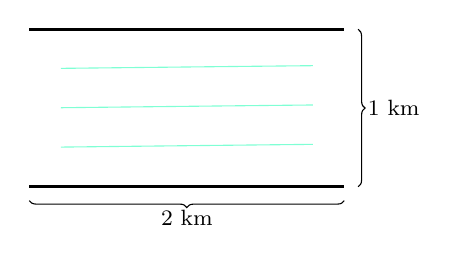
\begin{tikzpicture}[scale=2]
      \draw[very thick] (0,0) -- (2,0);
      \draw[very thick] (0,1) -- (2,1);
      \draw[decorate, decoration={brace, raise=5pt}] (2,0) -- (0,0)
        node[midway, below=5pt] {\footnotesize \(2\) km};
      \draw[decorate, decoration={brace, raise=5pt, mirror}] (2,0) -- (2,1)
        node[midway, right=5pt] {\footnotesize \(1\) km};
      \draw[Aquamarine, domain=0.2:1.8, smooth, samples=100] plot ({\x},{sin(4*pi*\x)*0.05+0.75});
      \draw[Aquamarine, domain=0.2:1.8, smooth, samples=100] plot ({\x},{sin(4*pi*\x)*0.051+0.50});
      \draw[Aquamarine, domain=0.2:1.8, smooth, samples=100] plot ({\x},{sin(4*pi*\x)*0.051+0.25});
    \end{tikzpicture}
    \blanklines{42}
  \end{example}

  Sometimes, we have to uncover hidden information. 

  \begin{example}
    A haunted house is trying to maximize revenue for next year. This year, if the ticket price was \textdollar{20}, then the average attendance was \(500\) visitors per evening. If the ticket price was \textdollar{15}, then the average attendance was \(800\) visitors per evening.  Assume average visitor per evening is linearly related to ticket price.

    Find the ticket price that maximizes revenue per evening. 
    \blanklines{48}
  \end{example}
  \clearpage

  \textbf{The general optimization strategy with some additional comments.}
  \label{page:optimization-strategy}
  \begin{enumerate}[label=(\arabic*)]
    \item Sketch the given scenario and \emph{introduce variables}. Make sure every variable measures something.

      \hlsupp{Common misadventure(s) at this step?}
      \begin{itemize}
        \item The sketch and its labels are inaccurate. If undetected, it is relatively challenging to recovers from this mistake. Be sure to double-check the sketch.
        \item Measure the wrong quantity (or quantities). If this happens, we most likely will not be able to eliminate all but one independent variable in step (4).
      \end{itemize}

    \item Identify the \hlwarn{objective variable}. Write ``\emph{\hlattn{Goal: We want to minimize/maximize \ldots{}}}.''

      \hlsupp{Common misadventure(s) at this step?}
      \begin{itemize}
        \item Misread the question and sought to maximize instead of minimize (or the other way around). 
      \end{itemize}


    \item Use the given scenario and our earlier sketch to figure out the \hlmain{relation} among our variables. Write down function(s), equation(s) and whatever it takes to fully describe the scenario in mathematical terms. In this step, we typically end up with one or more equations. Sometimes, we have to uncover hidden information.

      \hlsupp{Common misadventure(s) at this step?}
      \begin{itemize}
        \item Forgetting one or more relations is often the problem. If this happens, we most likely will not be able to eliminate all but one independent variable in step (4).
        \item If we measured the wrong quantity (or quantities) in step (1), then some quantities are not related to the rest. If this happens, then go back to step (1) and try again.
      \end{itemize}

    \item Treat the objective variable as the dependent variable and all other variables as independent. Eliminate all but one independent variable, so that the objective variable is a single-variable function in the remaining variable.

      \hlsupp{Common misadventure(s) at this step?}
      \begin{itemize}
        \item If we cannot eliminate all but one independent variable, then check for mistakes in steps (1) and (3).
        \item Algebra mistakes can also happen here.
        \item Sometimes, especially when we are stressed or under time pressure, we eliminate the objective variable away. That's why step (2) is important. Always make sure we know what the goal is.
      \end{itemize}

    \item \hlattn{Achieve the goal we wrote down in step (2)} using techniques from previous sections.

      Sometimes, it could be very hard to achieve our goals \emph{directly}. In such case, we try to achieve a related goal but more directly achievable goal and infer the required the extrema. 

      More precisely, if the extrema of a function \(f(x)\) is hard to find, but the extrema of a related function \(g(x)\) can be found much easier, AND at a number \(c\), \(f(c)\) and \(g(c)\) are both maxima (or both minima), then we find \(c\) by maximizing/minimizing \(g(x)\) instead. Note it does not mean \(g(c) = f(c)\).
      Example~\ref{ex:optimization-swim} demonstrates this idea.
  \end{enumerate}
  \clearpage

  \begin{example} \label{ex:optimization-ladder}
    Suppose a \(2\)-metre tall fence stands \(1\) metre away from a tall wall.  What is the shortest ladder that will reach over the fence to the wall.
    \blanklines{54}
  \end{example}

  \begin{example}
    Find the point on the circle \(x^{2} + 4y^{2} = 1\) that is closest to the point \((1,-2)\).
    \blanklines{55}
  \end{example}

  \begin{example}
    Take standard printer paper which has dimension \(8.5 \times 11\) inches. We want to fold it down the middle of the long side (and parallel to the short side) to create a prism shape. Assume the two ends of the prism are sealed. What is the angle between the two folded sides that maximizes the volume of the resulting prism?

    \blanklines{45}

    \faComment{} What if the paper is \(1094379843\) cm wide and \(47839274932\) cm long? What angle maximizes the volume? Does the dimension of the paper matter at all?
  \end{example}
\end{lesson}
\end{document}
